
\documentclass{article}
 \usepackage{graphicx}
\setlength{\parindent}{0em}
\setlength{\parskip}{1em}
\title{Proof of Concept - Elaboration}
\author{Osmond Chiu}


\begin{document}
\maketitle
\section*{Planned Thesis Topic}

My planned thesis research will be inductive research that aims to understand re-nationalisations in Australia. Re-nationalisations are when privatised government functions are brought back under public ownership.\par
The aim is to work out why these re-nationalisations occurred through compiling a list of re-nationalisations to identify common factors and examining key case studies.

\section*{Computational Analysis}
\subsection*{Decomposing}
There are a range of discrete tasks for this job. It will involve breaking rgw job down into:
\begin{itemize}
    \item defining what data needs to be collected
    \item determining the available resources to conduct the research
    \item conducting the research
    \item collecting the data
    \item organising the collected data
    \item analysing the collected data
    \item determining if the process needs to be repeated
\end{itemize}

\subsection*{Pattern Recognition}
There will be some recurring patterns in how I organise the collected data including metadata and tagging sources.\par

\subsection*{Algorithm}
Step-by-step, this job would likely involve:
\begin{enumerate}
\item Defining the research aim
\item Determining parameters such as time period, location and keywords for research
\item Identifying available sources and databases
\item Researching what tools interact with those sources and databases
\item Testing the tools
\item Using the tool, if it works
\item Saving sources
\item Producing metadata
\item Organising sources
\item Analysing sources
\item Deciding if the process needs to be repeated because the research aim is not met
\end{enumerate}

\section*{Elaboration}

There are a range of technologies that could help deliver the step-by-step requirements listed in my algorithm.

\subsection*{Requirements}

Of the steps outlined, the following steps could be improved with tools:
\begin{itemize}
\item Using a tool to better interact with sources and databases
\item organising saved sources
\item analysing sources 
\end{itemize}\par

The requirement for the first step might be tools that can conduct a search for different keywords in documents as the term "re-nationalisation" is not always used. The sources are most likely to primarily be newspaper articles.\par
\par
Analysing sources might require being able to do a text analysis of sources to determine what keywords are used and whether there are any patterns that can be identified across multiple sources about re-nationalisation.
\par
Requirements for organising sources might be a tool to tag and keep notes for each source Without having to re-read sources, enabling a de facto annotated bibliography.
\par

\subsection*{Data Collection}
\subsubsection*{Objective}

The first requirement could be met by using a tool to capture newspaper articles about examples of re-nationalisation in Australia from online archives.\par

The use of Application Programming Interfaces (APIs) to conduct searches within news aggregators may be the best way to deliver on that requirement. An API that could conduct searches on Factiva and ProQuest Australia and New Zealand Newsstream, narrowed to specific keywords in text and Australian newspaper sources would aid my research.\par

This may require writing some custom script to use the APIs to capture sources, export them and associated metadata.\par 

\subsubsection*{Mitigating risks}

There may be risks with data collection, for example, it is not immediately clear that some resources can use APIs such as Google Scholar. Identifying what resources have APIs that may be useful should be done first to know how much work must be done. Time may be wasted searching for and learning how to use tools to run scripts when there are no APIs.\par

There may be other difficulties automating such as copyright. Terms and Conditions of ProQuest and Factiva, which host more recent newspaper articles states that users shall not text mine or data mine. This information is at \begin{verbatim}https://libguides.mq.edu.au/textdatamining/publisher_resources\end{verbatim}

Finally, the risk may be that the tool does not find much information meaning it may have been a waste of time.\par

\subsubsection*{Result of Test}

I searched and was not able to locate any APIs for the news aggregators. Advice provided also indicated that ProQuest and Factiva do not have freely accessible APIs and would charge for their usage.

This means I will need to do manual searches using aggregators such as ProQuest, Factiva and Google Search. It will be necessary to keep track of search terms used by producing metadata.

\subsection*{Text Analysis}
\subsubsection*{Objective}

With difficulties in automating data collection, analysing the data may be an alternative. It would, however, first require manually collecting sources to feed into the tools.\par  

The second requirement may be met through using text analysis tools to analyse and visualise data. There are open source tool to conduct an open source, textual analysis such as Voyant or Gephi.

\subsubsection*{Mitigating risks}

The big risk may be that the tool does not produce any useful output from the included information meaning it was a waste of time. Testing it beforehand and understanding what kind of output may be generated will therefore be important. Examining the help documentation will assist, which is available for Voyant at https://voyant-tools.org/docs/\par

\subsubsection*{Result of test}

I decided to test Voyant to determine if text analysis would be useful for the analysis I would want. I chose Voyant as it did not require an installation unlike Gephi.

I tested the tool by uploading a three PDF articles on the reversal of the privatisation of the Port Macquarie Base Hospital to Voyant from ProQuest.

\begin{figure}[htp]
    \centering
    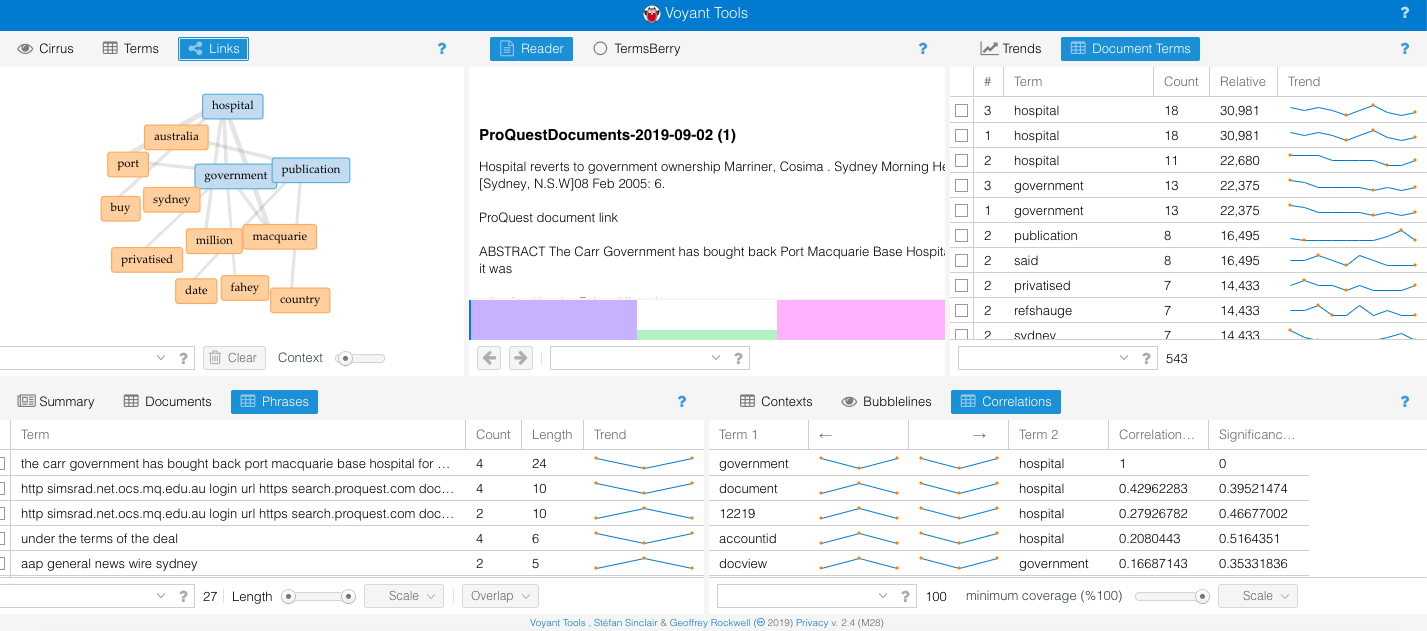
\includegraphics[width=10cm]{Voyant.png}
    \label{fig:voyant}
\end{figure}

The results highlighted the frequency of terms such as 'public', 'government' and 'privatised' but did not provide any useful insight about relationships. Given the language used and the number of sources available, it seems unlikely to provide any useful analysis about why re-nationalisation occurred. Analysis may require understanding the broader socio-economic context and reading between the lines.

\subsection*{Organising Data}
\subsubsection*{Objective}

The third requirement could be met by using a software that could organise, collect and keep information on sources. Ideally it would be able to tag themes, locate key terms, include notes and enable examining across multiple sources. There are a range of options that could be explored that include:

\begin{itemize}
\item NVivo - a qualitative data analysis tool that has plenty of functions but is not an open source tool meaning it may change or cost a significant sum 
\item Hypothes.is - a free online platform allowing annotatation, highlighting and tagging of web pages and PDF documents
\item Zotero - bibliographical software which allows tagging of sources and notes
\item Endnote - bibliographic software but not open source.
\item Ambar - software with a tagging and search capability but it will require a small payment or some script and other software to be installed
\item Open Semantic Desktop - software with a wider range of capabilities, tagging with full text search, exploratory search, analytics and text mining in many documents
\end{itemize}

\subsubsection*{Mitigating risks}

The main risk is not all tools have the same features. An incorrect choice could lead to a problem whereby a feature is not available, resulting in more work. It may be a case where multiple tools will need to be used and thus more time will to be spent learning how to use the tools. For example, Open Semantic Search has most features but not does appear to be a good reference manager for a thesis.\par 

It will be important to search for information comparing the features of different software and test the software for likely needs such as organising, tagging, citations, annotating sources before its use.\par

\subsubsection*{Result of test}

Of the available options, Open Semantic Search was tested as it had the most features covered off (tagging, search, text analysis). Hypothes.is was also tested as a less complex, alternative albeit with no offline function.

\begin{figure}[htp]
    \centering
    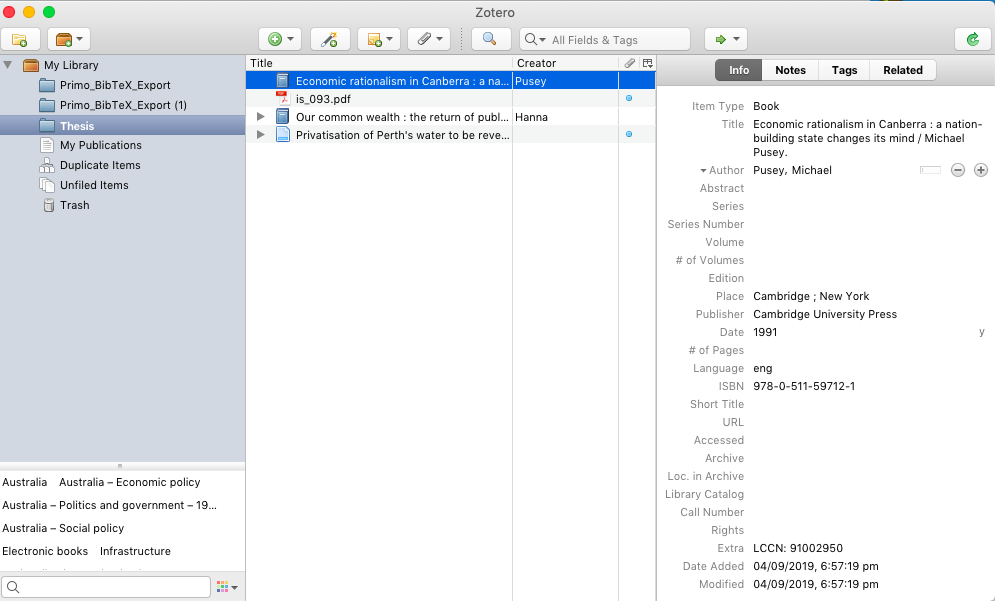
\includegraphics[width=10cm]{OpenSemantic.png}
    \label{fig:opensemantic}
\end{figure}

Open Semantic Search required the download and installation of a VirtualBox program for it to work. A few installation and access issues were resolved with advice from other websites, however, I was not able to use the program. The Solr search server never fully loaded and was lagging. It may be a technological issue as I am using a older laptop.

\begin{figure}[htp]
    \centering
    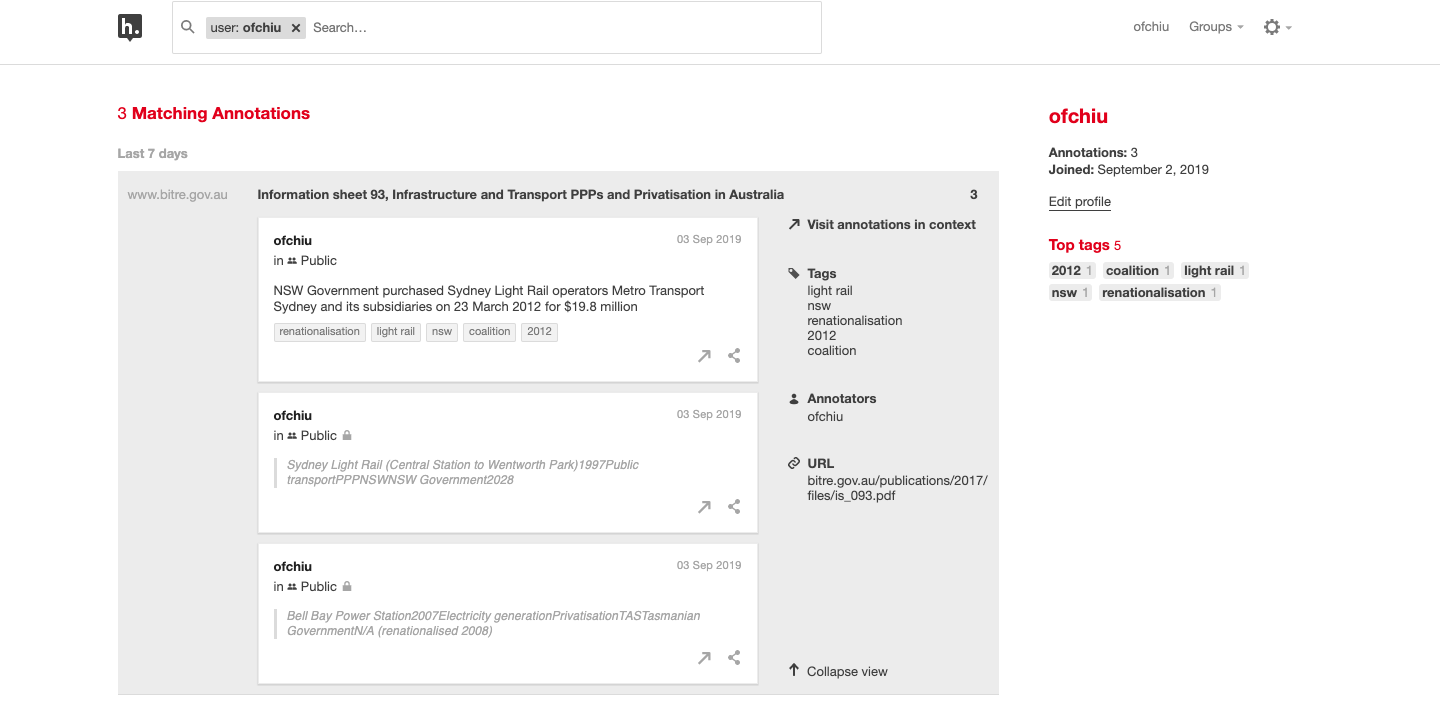
\includegraphics[width=10cm]{Hypothesis.png}
    \label{fig:hypothesis}
\end{figure}

The alternative option of Hypothes.is only required the installation of a browser add-on or use of bookmarking and the creation of an account. Tests of highlights, annotations and tags on a PDF and webpages were successful with the information transferred across. Hypothes.is is limited to online sources which limits its use for any downloaded documents.

There did not appear to be a bibliography or referencing feature in Hypothes.is which would be needed. A tool like bibliography software might be useful to fill this gap because the organisation of data will need to consider referencing during the research process, not at the end of the process. Zotero was chosen for testing because it was an open source option with integration with Word and LaTex.

\begin{figure}[htp]
    \centering
    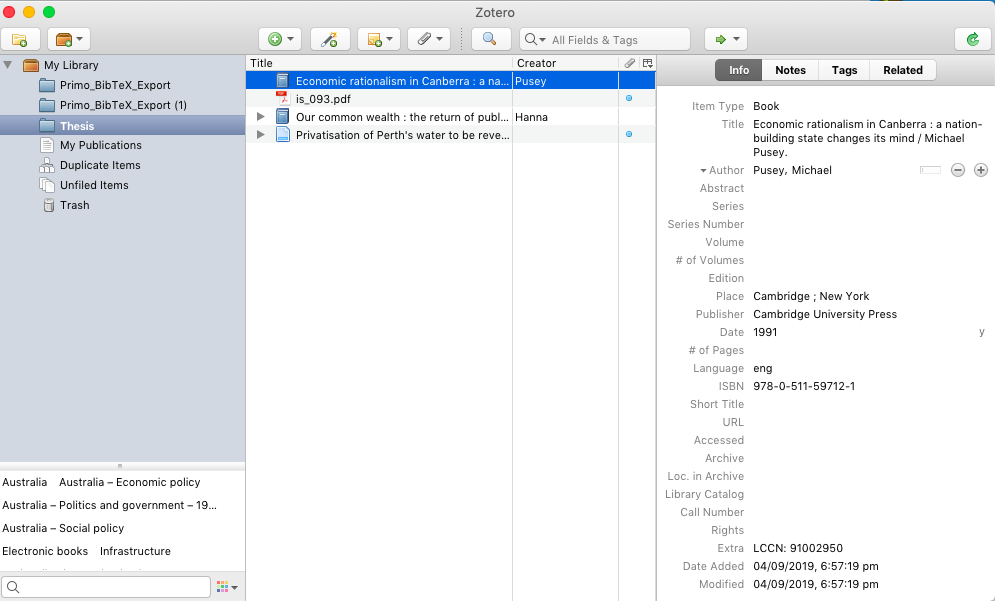
\includegraphics[width=10cm]{Zotero.png}
    \label{fig:zotero}
\end{figure}

Zotero was tested using imported Bibtex files from the MAcquarie University Library website and also the browser integration for HTML and PDF files. Tags and notes for references were included. This occurred without major problems, however, manual cleaning of titles will be likely. It was also not clear how data could easily migrate between Zotero and Hypothes.is.

\subsection*{Conclusion}

My elaboration has identified that improving the organisation of data is where tools could aid the most. Text analysis did not prove to be useful and data collection will need to be done manually as there are no APIs in news aggregators.

A combination of Hypothes.is and Zotero can be used to improve the organisation of data without significant issues. The tagging of offline documents will not be addressed using these two tools and the transferring of references between the two will involve some manual work. There are other tools with more features that may allow other options but these two will cover the most ground with the least number of technical issues.


\end{document}